% Metódy inžinierskej práce

\documentclass[10pt,twoside,slovak,a4paper]{article}

\usepackage[slovak]{babel}
\usepackage{pdfpages}
%\usepackage[T1]{fontenc}
\usepackage[IL2]{fontenc} % lepšia sadzba písmena Ľ než v T1
\usepackage[utf8]{inputenc}
\usepackage{graphicx}
\usepackage{dirtytalk}
\usepackage{url} % príkaz \url na formátovanie URL
\usepackage{hyperref} % odkazy v texte budú aktívne (pri niektorých triedach dokumentov spôsobuje posun textu)

\usepackage{cite}
%\usepackage{times}

\pagestyle{headings}

\title{Tvorba softvéru pomocou umelej inteligencie
\thanks{Semestrálny projekt v predmete Metódy inžinierskej práce, ak. rok 2021/22, vedenie: Ing. Vladimír Mlynarovič}} % meno a priezvisko vyučujúceho na cvičeniach

\author{Ľubomír Novotný\\[2pt]
	{\small Slovenská technická univerzita v Bratislave}\\
	{\small Fakulta informatiky a informačných technológií}\\
	{\small \texttt{xnovotnyl1@stuba.sk}}
	}

\date{\small 1. október 2021} % upravte



\begin{document}

\maketitle

\begin{abstract}

Pri tvorbe a udržiavaní softvéru nám umelá inteligencia môže podstatne pomôcť. Tento článok sa zaoberá využitím umelej inteligencie pri testovaní softvéru, najmä používateľského rozhrania. Používateľské rozhranie testované softvérom riadeným udalosťami (event driven software testing) môže ťažiť z využitia AI riešení. Umelá inteligencia výrazne pomohla procesu automatizácie rôznych softvérových procesov. Riešenia pomocou umelej inteligencie znižujú cenu a garantujú lepšiu kvalitu a dôkladné testovanie. Testovanie používateľského rozhrania sa môže pokladať za najnáročnejšiu časť testovania softvéru. Hoci výsledky sú dosť predbežné, ale aplikovanie rôznych AI techník pre testovanie používateľského rozhrania preukázalo prínos ideálnych výsledkov.
\end{abstract}

\section{Úvod}

Umelá inteligencia je nový prelom v oblasti informatiky~\ref{AI}. Umelá inteligencia má veľký vplyv v posledných rokoch na naše postupy pri riešení problémov ale aj na naše každodenné životy. AI používa počítače na riešenie inak neriešiteľných problémov a zlepšenie kvality dočasných počítačových systémov. Dôležitou otázkou je, či môžeme priamo použiť AI na problémy softvérového inžinierstva~\ref{SWE}, a či procesy softvérového inžinierstva sú schopné využiť umelú inteligenciu~\ref{pouzitie AI pri SW}.
Testovanie a podobné aktivity si vyžadujú veľa pozornosti počas celej fázy tvorby softvéru, aby sme mohli vytvoriť požadovaný softvér. Na tento zdĺhavý a komplikovaný problém môžeme použiť umelú inteligenciu.  Umelá inteligencia je schopná vykonávať širokú škálu činností, ktoré by inak neboli možné naprogramovať konvenčným spôsobom. Testovanie používateľského rozhrania je podobné rôznym iným činnostiam, ktoré sme dokázali vyriešiť pomocou umelej inteligencie. V posledných rokoch boli možnosti umelej inteligencie vyšetrované, a bola použitá na automatizáciu testovania softvéru.

\section{Softvérové inžinierstvo} \label{SWE}
Softvérové inžinierstvo sa zaoberá tvorbou softvérových systémov ale aj efektivitu softvérových systémov. Efektivita je dôležitá, pretože v reálnom svete mame na vývoj a údržbu ohraničené zdroje , stanovené požiadavky a časový limit. Preto môžeme povedať že softvérové inžinierstvo sa zaoberá tvorbou väčších softvérových systémov čo najefektívnejším spôsobom. Pri tvorbe sa sústreďujeme na tvorbu čo najspoľahlivejšieho softvéru, pričom sa snažíme čo najlepšie využiť schopnosti softvérových inžinierov.
Tvorbu softvéru môžeme realizovať rôznymi spôsobmi. Všetky procesy tvorby softvéru sa vykonávajú v jednotlivých etapách. Tie môžeme nazvať aj ako životný cyklus softvéru. Poznáme viacero takýchto modelov alebo životných cyklusov, ktorými sa môžeme riadiť pri tvorbe softvéru.\cite{swemb}
\begin{itemize}
    \item \textbf{Vodopádový model} je založený na jednoznačnom vymedzení činností, ktoré na seba nadväzujú a neprelínajú sa. Je vymedzená postupnosť krokov ktoré  za sebou nasledujú. Po poslednom kroku máme náš projekt dokončený.
    \item \textbf{Agilný model} je protikladom vodopádového modelu. Uplatňuje sa v projektoch, u ktorých je jasný cieľ, ale nedokážeme presne určiť detailný plán projektu bez priebežných prototypov. Agilný model je je interaktívny, pružný a prírastkový. Je závislý na častej spätnej väzbe počas procesu tvorby  prototypovania. Nastavujeme si stále nové požiadavky a parametre na základe a skúseností z jednotlivých iterácií. 
\end{itemize}
\cite{swemb}
\begin{center}
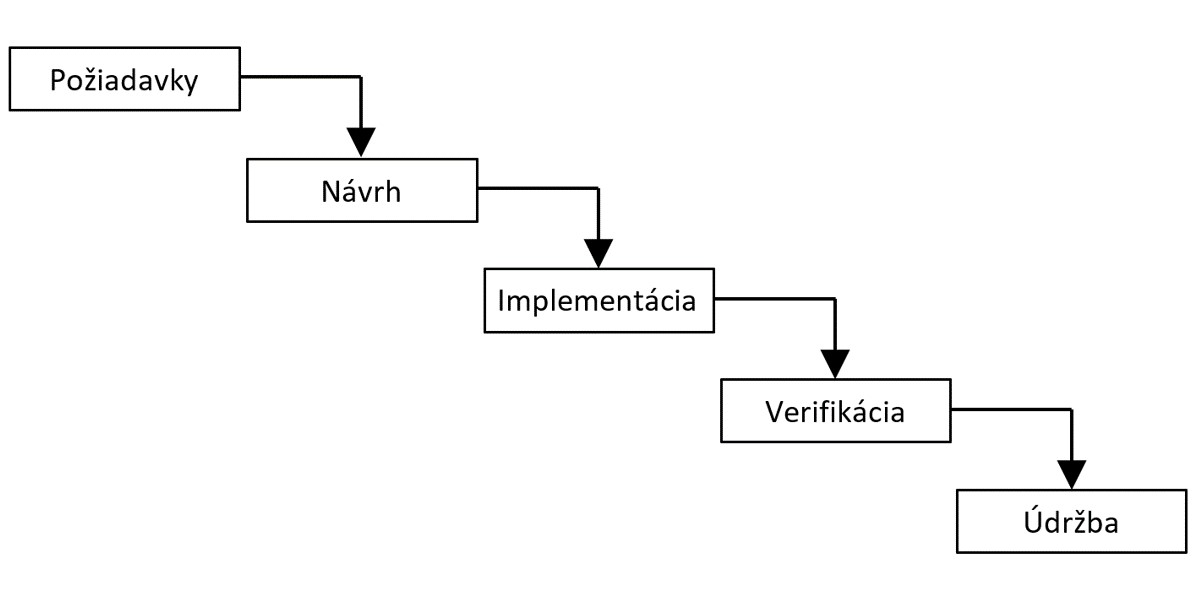
\includegraphics[scale=0.6]{vodopad1}
Obr. 1 Vodopádový model tvorby softvéru.
\end{center}


\subsection{Testovanie softvéru} \label{testovanie}
\say{Testovateľnosť: úsilie, ktoré treba vynaložiť na testovanie vlastností výrobku, napr. či vykazuje požadované správanie.}\cite{swemb}
Testovanie programu začína už na začiatku vývoja, keď samotný programátori testujú funkčnosť počas programovania. Konečné testovanie časti softvéru by nemal vykonávať tvorca softvéru, a malo by sa vykonávať systematicky, aby sa testovaním podrobila čo najväčšia časť programu. Testovanie je pomerne zložitá ale dôležitá oblasť, preto sa testovaniu venuje odborník, a nie programátor.\cite{CSEroadmap}
Pri samotnom procese testovania sa softvéroví inžinieri sústreďujú na celý životný cyklus testovania, ktorý začína testovaním funkcií a končí preberacím testovaním a zahŕňa:
\begin{itemize}
	\item Testy funkcií a modulov, ktoré sú vykonávané prevažne softvérovými inžiniermi priamo v etape implementácie.
	\item Integračné testy, čo je vlastne testovanie viacerých modulov súčasne.
			  \item Nezávislé testy - vykonávané nezávislými externými subjektami.
    \item Inštalačné testy - zahŕňajúce všeobecnú výkonnosť systému, ktorý je prvýkrát nainštalovaný na konkrétnom HW a operačnom systéme.
    \item Validačné testovanie – slúži k overeniu, že softvér spĺňa „rozumné očakávania“ zákazníka, ktoré sú definované v špecifikovaných požiadavkách.
    \item Preberacie testovanie - je to vlastne posledný míľnik pri testovaní projektu. V prípade úspešného zvládnutia nastáva oficiálne prevzatie projektu zákazníkom. Chyby môžu byť do aplikácie vnesené v každom štádiu životného cyklu vývoja aplikácie, vrátane testovania.
\end{itemize}
\cite{testovanie}
.Vodopádový spôsob vývoja softvéru sa spolieha na testovanie softvéru až po dokončení dizajnu, kódovania a splnenia podmienok. Agilný a iteratívny prístup tvorby softvéru predstavili prototypovanie, ktoré je použité na overenie požiadavok a verifikáciu minulej iterácie. Neustála verifikácia sa snaží využiť verifikácie zahŕňajúce formálne metódy a inšpekcie počas procesu tvorby, narozdiel od testovacej fázy na konci vývojovej fázy.\cite{CSEroadmap}

\section{Umelá inteligencia}\label{AI}

Pod umelou inteligenciou chápeme softvér, ktorý napodobňuje ľudské kognitívne funkcie tým, že má schopnosť učiť sa a riešiť problémy. Program sa správa tak, že ak by to robil človek, považovali by sme ho za inteligentného. Okrem rozpoznávania reči, obrazov, prekladu do jazykov dokáže imitovať rozmýšľanie ľudí - učiť sa, uvažovať, riešiť problémy, sám hľadať spôsoby, ako sa dostať k cieľu. Je to aj schopnosť počítačov používať algoritmus na učenie sa z dát a získané vedomosti použiť na rozhodovanie podobné ľudskému. Umelá inteligencia ako celok stavia vo veľkej miere na základoch mnohých ďalších vedných odborov, a to predovšetkým na informatike, matematike, štatistike, logike, lingvistike či neurovedách. Podobnosť umelej a ľudskej inteligencie je ale iba povrchná a nie je správne ich stotožňovať. Koncepcia ľudskej inteligencie je stále predmetom výskumu.
V súčasnosti sú k dispozícii iba algoritmy slabej inteligencie, špecializované na jedinú úlohu
(rozpoznávanie objektov, vrátane tváre, rozpoznávanie reči (virtuálne asistentky), prevod
medzi hovoreným a tlačeným textom,...). V súčasnosti sú algoritmy UI silné hlavne v rozpoznávaní obrazov, v analýze hovoreného slova, v analýze textu, v analýze štruktúrovaných a neštruktúrovaných dát a v podpore rozhodovania. Vďaka senzorom a kamerám UI vie „vidieť“, „počuť“, „čítať“. To všetko navyše rýchlo a v reálnom čase.\cite{AIvMed}


\section{Softvér používajúci umelú inteligenciu} \label{AISW}

%\paragraph{Veľmi dôležitá poznámka.}
%Niekedy je potrebné nadpisom označiť odsek. Text pokračuje hneď za nadpisom.

\section{Používanie AI pri tvorbe SW} \label{pouzitie AI pri SW}

\section{Záver} \label{zaver} % prípadne iný variant názvu

%\acknowledgement{Ak niekomu chcete poďakovať\ldots}

% týmto sa generuje zoznam literatúry z obsahu súboru literatura.bib podľa toho, na čo sa v článku odkazujete
\bibliography{literatura}
\bibliographystyle{plain} 
\end{document}
